\section{Semantics}
\label{sec:semantics}

% \section{Ordering and Type Safety}
% \label{sec:ordering}

We introduce and explore using \emph{synchronization schemas}~\citeMain{pods21},
and \emph{data-trace types}~\citeMain{festschrift18,pldi19,oopsla20}
to solve the problem of encoding ordering requirements in stream processing
systems.
These date back to Mazurkiewicz traces, studied in concurrency theory to model distributed sets of events~\cite{mazurkiewicz1986trace,DiekertR1995}.
These give a kind of semantics to stream processing programs (what it means for
them to be correct) in the presence of out-of-order data.
We also aim to answer the question: what are these types good for?
We explore their use as a programming discipline~\citeMain{pldi19},
implemented on top of Apache Storm~\cite{Storm},
as well as a lightweight testing technique~\citeMain{oopsla20},
implemented on top of Apache Flink~\cite{Flink}.

In this section, we describe the work based on data trace types~\citeMain{pldi19}.
Our ongoing work generalizes the data-trace types framework to
the symbolic setting with key-based partitionining and focuses on series-parallel streams~\citeMain{pods21}.

\subsection{Types for Data Streams}
\label{subsec:dtt-1}

A \defn{data type} $A = (\Sigma,(T_\sigma)_{\sigma \in \Sigma})$ consists of a potentially infinite \emph{tag alphabet} $\Sigma$ and a value type $T_\sigma$ for every tag $\sigma \in \Sigma$. The set of \emph{elements} of type $A$, or \defn{data items}, is equal to $\{ (\sigma,d) \mid \text{$\sigma \in \Sigma$ and $d \in T_\sigma$} \}$, which we will also denote by $A$. The set of \emph{sequences} over $A$ is denoted as $A^*$. A \defn{dependence relation} on a tag alphabet $\Sigma$ is a symmetric binary relation on $\Sigma$. We say that the tags $\sigma$, $\tau$ are \emph{independent} (w.r.t.\ a dependence relation $D$) if $(\sigma,\tau) \notin D$. For a data type $A = (\Sigma,(T_\sigma)_{\sigma \in \Sigma})$ and a dependence relation $D$ on $\Sigma$, we define the dependence relation that is induced on $A$ by $D$ as
$\{
   ((\sigma,d),(\sigma',d')) \in A \times A \mid
   (\sigma,\sigma') \in D
 \}
$,
which we will also denote by $D$. Define $\eq_D$ to be the smallest congruence (w.r.t.\ sequence concatenation) on $A^*$ containing $\{ (ab,ba) \in A^* \times A^* \mid (a,b) \notin D \}$. Informally, two sequences are equivalent w.r.t.\ $\eq_D$ if one can be obtained from the other by repeatedly commuting adjacent items with independent tags.

\begin{example}
\label{ex:dependence}
Suppose we want to process a stream that consists of sensor measurements and special symbols that indicate the end of a one-second interval. The data type for this input stream involves the tags $\Sigma = \{ \tg M, \tg\# \}$, where $\tg M$ indicates a sensor measurement and $\tg\#$ is an end-of-second marker. The value sets for these tags are $T_{\tg M} = \Nat$ (the natural numbers), and $T_{\tg\#} = \Ut$ is the unit type (singleton). So, the data type $A = (\Sigma,T_{\tg M},T_{\tg\#})$ contains measurements $(\tg M, d)$, where $d$ is a natural number, and the end-of-second symbol $\tg\#$.

The dependence relation $D = \{ (\tg M, \tg\#), (\tg\#, \tg M), (\tg\#,\tg\#) \}$ says that the tag $\tg M$ is independent of itself, and therefore consecutive $\tg M$-tagged items are considered unordered. For example, $(\tg M, 5) \; (\tg M, 5) \; (\tg M, 8) \; \tg\# \; (\tg M, 9)$ and $(\tg M, 8) \; (\tg M, 5) \; (\tg M, 5) \; \tg\# \; (\tg M, 9)$ are equivalent w.r.t.\ $\eq_D$.
\end{example}

A \defn{data-trace type} is a pair $X = (A,D)$, where $A$ is a data type and $D$ is a dependence relation on the tag alphabet of $A$. A \defn{data trace} of type $X$ is a congruence class of the relation $\eq_D$. We also write $X$ to denote the set of data traces of type $X$. Since the equivalence $\eq_D$ is a congruence w.r.t.\ sequence concatenation, the operation of concatenation is also well-defined on data traces: $[u] \cdot [v] = [uv]$ for sequences $u$ and $v$, where $[u]$ is the congruence class of $u$. We define the relation $\leq$ on the data traces of $X$ as a generalization of the prefix partial order on sequences: for data traces $\trc u$ and $\trc v$ of type $X$, $\trc u \leq \trc v$ iff there are $u \in \trc u$ and $v \in \trc v$ s.t.\ $u \leq v$ (i.e., $u$ is a prefix of $v$). The relation $\leq$ on data traces of a fixed type is a partial order. Since it generalizes the prefix order on sequences (when the congruence classes of $\eq_D$ are singleton sets), we will call $\leq$ the \emph{prefix order} on data traces.

\begin{example}[Data Traces]
\label{ex:data-trace}
Consider the data-trace type $X = (A,D)$, where $A$ and $D$ are given in Example~\ref{ex:dependence}. A data trace of $X$ can be represented as a sequence of multisets (bags) of natural numbers and visualized as a partial order on that multiset. The trace corresponding to the sequence of data items
$
  (\tg M, 5) \; (\tg M, 7) \; \tg\# \; (\tg M, 9) \; (\tg M, 8) \; (\tg M, 9) \; \tg\# \; (\tg M, 6)
$
is visualized as:
\newline
\centerline{\small
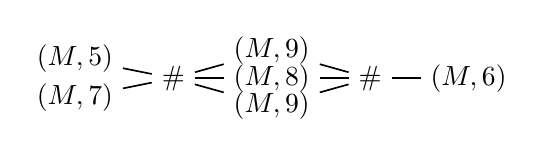
\begin{tikzpicture}[-, >=to, auto, node distance=1.25cm, semithick, transform shape]
\node (M1) {};
\node (T1) [above of=M1, node distance=0.25cm] {$(\tg M,5)$};
\node (B1) [below of=M1, node distance=0.25cm] {$(\tg M,7)$};
\node (M2) [right of=M1] {$\tg\#$};
\node (M3) [right of=M2] {$(\tg M,8)$};
\node (T3) [above of=M3, node distance=0.35cm] {$(\tg M,9)$};
\node (B3) [below of=M3, node distance=0.35cm] {$(\tg M,9)$};
\node (M4) [right of=M3] {$\tg\#$};
\node (M5) [right of=M4] {$(\tg M,6)$};
%
\path (T1) edge (M2);
\path (B1) edge (M2);
\path (M2) edge (T3);
\path (M2) edge (M3);
\path (M2) edge (B3);
\path (T3) edge (M4);
\path (M3) edge (M4);
\path (B3) edge (M4);
\path (M4) edge (M5);
\end{tikzpicture}
}%
\vspace{-1ex}
\newline
where a line from left to right indicates that the item on the right must occur after the item on the left. The end-of-second markers $\tg\#$ separate multisets of natural numbers. So, the set of data traces of $X$ has an isomorphic representation as the set $\Bag(\Nat)^+$ of nonempty sequences of multisets of natural numbers. In particular, the empty sequence $\epsilon$ is represented as $\emptyset$ and the single-element sequence $\tg\#$ is represented as $\emptyset \; \emptyset$.
\end{example}

A singleton tag alphabet can be used to model sequences or multisets over a basic type of values. For the data type given by $\Sigma = \{\sigma\}$ and $T_\sigma = T$ there are two possible dependence relations for $\Sigma$, namely $\emptyset$ and $\{(\sigma,\sigma)\}$. The data traces of $(\Sigma,T,\emptyset)$ are multisets over $T$, which we denote as $\Bag(T)$, and the data traces of $(\Sigma,T,\{(\sigma,\sigma)\})$ are sequences over $T$.

\begin{example}[Multiple Input/Output Channels]
\label{ex:channels}
Suppose we want to model a streaming system with multiple independent input and output channels, where the items within each channel are linearly ordered but the channels are completely independent. This is the setting of (acyclic) \emph{Kahn Process Networks} ~\cite{gilles1974semantics} and the more restricted synchronous dataflow models \cite{lee1987synchronous, benveniste2003synchronous}. We introduce tags $\Sigma_\tg{I} = \{ \tg{I}_1, \ldots, \tg{I}_m \}$ for $m$ input channels, and tags $\Sigma_\tg{O} = \{ \tg{O}_1, \ldots, \tg{O}_n \}$ for $n$ output channels.
The dependence relation for the input consists of all pairs $(\tg{I}_i,\tg{I}_i)$ with $i = 1, \ldots, m$. This means that for all indexes $i \neq j$ the tags $\tg{I}_i$ and $\tg{I}_j$ are independent. Similarly, the dependence relation for the output consists of all pairs $(\tg{O}_i,\tg{O}_i)$ with $i = 1, \ldots, n$. Assume that the value types associated with the input tags are $T_1$, \ldots, $T_m$, and the value types associated with the output tags are $U_1$, \ldots, $U_n$. The sets of input and output data traces are (up to a bijection) $T^*_1 \times \cdots \times T^*_m$ and $U^*_1 \times \cdots \times U^*_m$ respectively.
\end{example}

\subsection{Type-Consistent Programming}
\label{subsec:dtt-2}

Data-trace types are useful for giving the meaning (semantics) of a stream processing system. Consider the analogy with a functional model of computation: the meaning of a program consists of the input type, the output type, and a mapping that describes the input/output behavior of the program. Correspondingly, the semantics for a stream processing systems consists of:
\begin{enumerate}
\item
the type $X$ of input data traces,
\item
the type $Y$ of output data traces, and 
\item
a monotone mapping $\beta: X \to Y$ that specifies the cumulative output after having consumed a prefix of the input stream.
\end{enumerate}
The monotonicity requirement captures the idea that output items cannot be retracted after they have been omitted. Since $\beta$ takes an entire input history (data trace) as input, it can model stateful systems, where the output that is emitted at every step depends potentially on the entire input history.

We have already discussed how (monotone) functions from $A^*$ to $B^*$ model sequential stream processors. We will now introduce the formal notion of \emph{consistency}, which captures the intuition that a sequential implementation does not depend on the relative order of any two elements unless the stream type considers them to be relatively ordered.

\begin{definition}[Consistency]
Let $X = (A,D)$ and $Y = (B,E)$ be data-trace types. We say that a data-string transduction $f: A^* \to B^*$
is \emph{$(X,Y)$-consistent} if $u \eq_D v$ implies that $\bar{f}(u) \eq_{E} \bar{f}(v)$ for all $u, v \in A^*$.

Let $f \in A^* \to B^*$ be a $(X,Y)$-consistent data-string transduction. The function $\beta: X \to Y$, defined by
$\beta([u]) = [\bar f(u)]$ for all $u \in A^*$, is called the \emph{$(X,Y)$-denotation} of $f$.
\end{definition}

\begin{definition}[Data-Trace Transductions]
Let $X = (A,D)$ and $Y = (B,E)$ be data-trace types. A \textbf{\em data-trace transduction} with input type $X$ and output type $Y$ is a function $\beta: X \to Y$ that is monotone w.r.t.\ the prefix order on data traces: $\trc u \leq \trc v$ implies that $\beta(\trc u) \leq \beta(\trc v)$ for all traces $\trc u, \trc v \in X$. 
\end{definition}

It is shown in \cite{festschrift18} that the set of data-trace transductions from $X$ to $Y$ is equal to the set of $(X,Y)$-denotations of all $(X,Y)$-consistent data-string transductions.

We define two kinds of \textbf{\em data-trace types} for streams of key-value pairs: \emph{unordered} types of the form $\Unord(K,V)$, and \emph{ordered} types of the form $\Ord(K,V)$. For a set of keys $K$ and a set of values $V$, let $\Unord(K, V)$ denote the type with alphabet $K \cup \{\tg\#\}$, values $V$ for every key, values $\Nat$ for the $\tg\#$ tag (i.e., marker timestamps), and dependence relation $\{ (\tg\#, \tg\#) \} \cup \{ (k,\tg\#), (\tg\#,k) \mid k \in K \}$. In other words, $\Unord(K, V)$ consists of data traces where the marker tags $\tg\#$ are linearly ordered and the elements between two such tags are of the form $(k,v)$, where $k \in K$ and $v \in V$, and are completely unordered. We define $\Ord(K, V)$ similarly, with the difference that the dependence relation also contains $\{ (k,k) \mid k \in K \}$. That is, in a data trace of $\Ord(K,V)$, elements with the same key are linearly ordered between $\tg\#$ markers, but there is no order across elements of different keys.

A \textbf{\em transduction DAG} is a tuple $(S,N,T,E,\to,\lambda)$ which represents a labelled directed acyclic graph, where: $S$ is the set of \emph{source vertices}, $T$ is the set of \emph{sink vertices}, $N$ is the set of \emph{processing vertices}, $E$ is the set of \emph{edges} (i.e., connections/channels), $\to$ is the \emph{edge relation}, and $\lambda$ is a \emph{labelling function}. The function $\lambda$ assigns: (1) a data-trace type to each edge, (2) a data-trace transduction to each processing vertex that respects the input/output types, and (3) names to the source/sink vertices. We require additionally that each source vertex has exactly one outgoing edge, and each sink vertex has exactly one incoming edge.

\begin{example}[Time-Series Interpolation]
\label{ex:IoT}
Consider a home IoT system where temperature sensors are installed at a residence. We wish to analyze the sensor time series to create real-time notifications for excessive energy loss through the windows. The sensor time series sometimes have missing data points, and therefore the application requires a pre-processing step to fill in any missing measurements using linear interpolation. We assume that the sensors first send their measurements to a hub, and then the hub propagates them to the stream processing system. The stream that arrives from the hub does not guarantee that the measurements are sent in linear order (e.g., with respect to a timestamp field). Instead, it produces synchronization markers every 10 seconds with the guarantee that all elements with timestamps $< 10 \cdot i$ have been emitted by the time the $i$-th marker is emitted. That is, the $i$-th marker can be thought of as a watermark with timestamp $10 \cdot i$. The input stream is a data trace of $\Unord(\Ut,\texttt{M})$, where $\texttt{M}$ is the type of measurements $(\mathit{id}, \mathit{value}, \mathit{ts})$ consisting of a sensor identifier $id$, a scalar value $value$, and a timestamp $ts$. This is a transduction DAG that describes the pre-processing computation:
\newline
\centerline{%
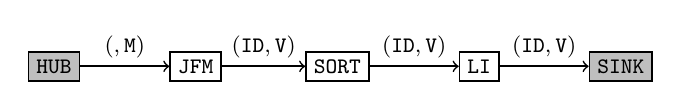
\begin{tikzpicture}[->, >=to, auto, node distance=1.8cm, semithick, transform shape]
%
\footnotesize
%
\node (A) [draw, fill=lightgray] {\texttt{HUB}};
\node (B) [draw, right of=A] {\texttt{JFM}};
\node (C) [draw, right of=B] {\texttt{SORT}};
\node (D) [draw, right of=C] {\texttt{LI}};
\node (E) [draw, fill=lightgray, right of=D] {\texttt{SINK}};
%
\path (A) edge node {$\Unord(\Ut,\texttt{M})$} (B);
\path (B) edge node {$\Unord(\texttt{ID},\texttt{V})$} (C);
\path (C) edge node {$\Ord(\texttt{ID},\texttt{V})$} (D);
\path (D) edge node {$\Ord(\texttt{ID},\texttt{V})$} (E);
%
\end{tikzpicture}
}% end of centerline
\newline
The vertex \texttt{HUB} represents the source of sensor measurements, and the vertex \texttt{SINK} represents the destination of the output stream. \texttt{ID} is the type of sensor identifiers, and \texttt{V} is the type of timestamped values $(\mathit{value}, \mathit{ts})$. The processing vertices are described below:
\begin{itemize}
\item
The stage Join-Filter-Map (\texttt{JFM}) joins the input stream with a table that indicates the location of each sensor, filters out all sensors except for those that are close to windows, and reorganizes the fields of the input tuple.
\item
Recall the guarantee for the synchronization markers, and notice that it implies the following property for the input traces: for any two input measurements that are separated by at least one marker, the one on the left has a strictly smaller timestamp than the one on the right. The sorting stage \texttt{SORT} sorts for each sensor the measurements that are contained between markers.
\item
The linear interpolation stage \texttt{LI} considers each sensor independently and fills in any missing data points.
\end{itemize}
We have described informally the data-trace transductions \texttt{JFM}, \texttt{SORT} and \texttt{LI}. The transduction DAG shown earlier denotes a data-trace transduction $\Unord(\Ut,\texttt{M}) \to \Ord(\texttt{ID},\texttt{V})$.
\end{example}

The computation performed by a processing node is given in a structured fashion, by completing function definitions of a specified \textbf{\em operator template}. Table~\ref{table:templates} shows the three templates that are supported, which encompass both ordered and unordered input streams. Each operator is defined by a sequential implementation, which we describe informally below. This means that each operator can be modeled as a data-string transduction. It can then be proved formally that these data-string transductions are consistent w.r.t.\ their input/output data-trace types. It follows that each operator that is programmed according to the template conventions has a denotation (semantics) as a data-trace transduction of the appropriate type.

\texttt{\bfseries OpStateless}:
The simplest template concerns \emph{stateless} computations, where only the current input event---not the input history---determines the output. The programmer fills in two function definitions: (1) \texttt{onItem} for processing key-value pairs, and (2) \text{onMarker} for processing synchronization markers. The functions have no output (the output type is \texttt{Ut}, i.e.\ the unit type) and their only side-effect is emitting output key-value pairs to the output channel by invoking $\texttt{emit(outputKey, outputValue)}$.

\texttt{\bfseries OpKeyedOrdered}:
Assuming that the input is ordered per key, this template describes a stateful computation for each key independently that is order-dependent. The programmer fills in three function definitions: (1) \texttt{initialState} for obtaining the initial state, (2) \texttt{onItem} for processing a key-value pair and updating the state, and (3) \texttt{onMarker} for processing a synchronization marker and updating the state. The functions have output $S$, which is the type of the data structure for representing the state. As for stateless computations, the functions allow the side-effect of emitting output key-value pairs to the output channel. This template requires a crucial \emph{restriction} for maintaining the order for the output: every occurrence of \texttt{emit} must preserve the input key. If this restriction is violated, e.g.\ by projecting out the key, then the output cannot be viewed as being ordered.

\texttt{\bfseries OpKeyedUnordered}:
Assuming that the input is unordered, this template describes a stateful computation for each key independently. Recall that the synchronization markers are ordered, but the key-value pairs between markers are \emph{unordered}. To guarantee that the computation does not depend on some arbitrary linear ordering of the key-value pairs, their processing does not update the state. Instead, the key-value pairs between two consecutive markers are aggregated using the operation of a \emph{commutative monoid} $A$: the programmer specifies an identity element $\texttt{id()}$, and a binary operation $\texttt{combine()}$ that must be \emph{associative} and \emph{commutative}. Whenever the next synchronization marker is seen, \texttt{updateState} is used to incorporate the aggregate (of type $A$) into the state (of type $S$) and then \texttt{onMarker} is invoked to (potentially) emit output. The behavior \texttt{onItem} may depend on the last snapshot of the state, i.e.\ the one that was formed at the last marker. The functions \texttt{onItem} and \texttt{onMarker} are allowed to emit output data items (but not markers), but the rest of the functions must be pure (i.e., no side-effects).

\begin{theorem}
\normalfont
Every streaming computation defined using the operator templates above is consistent w.r.t.\ its input/output type.
\end{theorem}
